%!TEX root=../GaugeCNNTheory.tex


\subsection{Azimuthal rotation equivariant spherical CNNs on cylindrical topologies}
\label{sec:spherical_CNNs_azimuthal_equivariant}



Besides fully $\SO3$ or $\O3$-equivariant spherical convolutions, many spherical CNNs are designed to be equivariant w.r.t. azimuthal rotations around a specified polar axis.
All of the models discussed in this section rely either on the $\SO2$-invariant $\{e\}$-structure
that is shown in Figs.~\ref{fig:G_structure_S2_2} and \ref{fig:spherical_equirectangular_1}
or, alternatively, that in Fig.~\ref{fig:spherical_equirectangular_2}.
Due to the triviality of the structure group $G=\{e\}$, the kernel spaces remain unconstrained ($\{e\}$-steerable).
Features are transported according to the unique $\{e\}$-compatible trivial connection which differs from the usual spherical Levi-Civita connection.
With this information, and with the explicit exponential maps in Eq.~\eqref{eq:sphere_expmap_explicit}, the spherical $\GM$-convolutions in this section are in theory fully specified.
In practice, the implementations, listed in row (34) of Table~\ref{tab:network_instantiations}, differ in their numerical implementations, which we discuss in the following.


\begin{SCfigure}
    \centering
    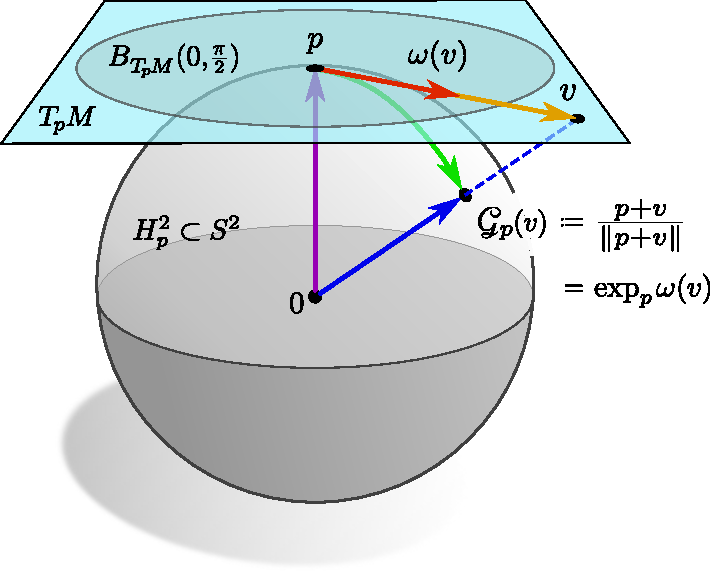
\includegraphics[width=.55\textwidth]{figures/gnomonic_proj.pdf}
    \captionsetup{width=1.02\textwidth}
    \hspace{1ex}
    \caption{\small
        Gnomonic projection ${\mathscr{G}_p\!: \TpM \to H_p^2}$ of the tangent space at $p$ to the upper hemisphere $H_p^2 \subset S^2$ around~$p$.
        When interpreting the sphere as being embedded in $\R^3$, the gnomonic projection $\mathscr{G}_p(v)$ (blue) is given by the sum of ${p\in S^2 \subset \R^3}$ (purple) and $v\in\TpM \subset\R^3$ (yellow) in ambient space, followed by a normalization back to the sphere.
        Theorem~\ref{thm:gnomonic} proves that this operation is equivalent to a projection of a radially warped vector $\omega(v) = \arctan(\lVert v\rVert) \frac{v}{\lVert v\rVert} \in B_{\TpM}(0,{\textstyle\frac{\pi}{2}})$ (red) via the exponential map (green).
        The gnomonic projection based spherical convolutions in
        \cite{coors2018spherenet,zhao2018distortion,tateno2018distortion,eder2019convolutions,martin2020panoramic}
        are therefore special cases of spherical $\GM$-convolutions with radially warped kernels.
        $\GM$-convolutions are more general since they allow for kernel projections over the whole sphere instead of the upper hemisphere only.
        \\\protect\rule{0ex}{0.ex}
    }
    \label{fig:gnomonic_proj}
\end{SCfigure}


Concurrent with our definition of convolutional weight sharing, the models in \cite{coors2018spherenet,zhao2018distortion,tateno2018distortion,eder2019convolutions,martin2020panoramic} share a given template kernel over the tangent spaces by orienting it relative to the frames of the considered $\{e\}$-structure in Fig.~\ref{fig:G_structure_S2_2}.
However, contrary to $\GM$-convolutions, the matching of these kernels with the feature field is not done via exponential maps (or transporter pullbacks), but via the gnomonic projection.
This gnomonic projection is at any point $p$ defined by
\begin{align}\label{eq:gnomonic_proj_def}
    \mathscr{G}_p:\, \TpM \to H_p^2, \quad v \mapsto \frac{p+v}{\lVert p+v\rVert} \,,
\end{align}
which is visualized in Fig.~\ref{fig:gnomonic_proj}.
The summation of $p\in S^2 \subset \R^3$ with tangent vectors $v \in \TpM \subset \R^3$ is hereby performed in the embedding space $\R^3$ and the normalization projects the result back to the sphere. %guarantees that the result lies on the sphere.
The codomain of the gnomonic projection is the ``upper'' hemisphere
\begin{align}\label{eq:upper_hemisphere_def}
    H_p^2 := \big\{ q\in S^2 \,\big|\, \langle p,q\rangle_{\R^3} > 0 \big\} \,\subset S^2
\end{align}
centered around $p$.
Given this difference in the kernel projections, it might seems like the models in \cite{coors2018spherenet,zhao2018distortion,tateno2018distortion,eder2019convolutions,martin2020panoramic} are not (or only approximately) explained as $\GM$-convolution.
The following theorem proves, however, that the gnomonic projection is equivalent to a projection via the exponential map after applying a \emph{radial warp}
\begin{align}\label{eq:radial_warp}
    \omega:\ \TpM \to B_{\TpM}(0,{\textstyle\frac{\pi}{2}}), \quad
    v \mapsto \arctan\! \big(\lVert v\rVert\big) \frac{v}{\lVert v\rVert}
\end{align}
to the tangent spaces, which contracts tangent vectors to an open ball of radius $\pi/2$ around the origin:
\begin{thm}[Gnomonic projections as warped exponential maps]
\label{thm:gnomonic}
    The gnomonic projection $\mathscr{G}_p$ of $\TpM$ to the upper hemisphere $H_p^2\subset S^2$, defined in Eq.~\eqref{eq:gnomonic_proj_def}, is equivalent to a projection of its radial warp $\omega(\TpM) = B_{\TpM}(0,{\textstyle\frac{\pi}{2}})$, Eq.~\eqref{eq:radial_warp}, via the exponential map, that is, the following diagram commutes:
    \begin{equation}\label{cd:gnomonic_exp_warp}
    \begin{tikzcd}[column sep=60, row sep=6pt, font=\normalsize]
        \TpM
            \arrow[dr, pos=.45, "\mathscr{G}_p"]
            \arrow[dd, "\omega\,"']
        \\
        & H_p^2 \subset S^2
        \\
        B_{\TpM}(0,{\textstyle\frac{\pi}{2}})
            \arrow[ur, pos=.3, "\exp_p"']
    \end{tikzcd}
    \end{equation}
    In equations,
    \begin{align}
        \mathscr{G}_p(v) \,=\, \exp_p \circ\, \omega(v)
    \end{align}
    holds for any $p\in S^2$ and any $v\in\TpM$.
\end{thm}
\begin{proof}
    The proof is given by the following simple calculation, which holds for any $p\in S^2$ and any $v\in \TpM$:
    \begin{align}
        \exp_p \circ\mkern2mu \omega (v)
        \ &\overset{(1)}{=}\ p\cdot \cos\! \big(\lVert \omega(v)\rVert\big) \,+\, \frac{\omega(v)}{\lVert \omega(v)\rVert}\cdot \sin\! \big(\lVert \omega(v)\rVert\big) \notag \\
        \ &\overset{(2)}{=}\ p\cdot \cos\! \big(\!\arctan(\lVert v\rVert)\big) \,+\, \frac{v}{\lVert v\rVert}\cdot \sin\! \big(\!\arctan(\lVert v\rVert)\big) \notag \\
        \ &\overset{(3)}{=}\ \frac{p+v}{\sqrt{1+\lVert v\rVert^2}} \notag \\
        \ &\overset{(4)}{=}\ \frac{p+v}{\lVert p+v\rVert} \notag \\
        \ &\overset{(5)}{=}\ \mathscr{G}_p(v)
    \end{align}
    The first two steps make use of the explicit definition of the embedded sphere's exponential map, Eq.~\eqref{eq:sphere_expmap_explicit}, and the radial warp, Eq.~\eqref{eq:radial_warp}.
    The third step follows since $\cos \circ \arctan(x) = \frac{1}{\sqrt{1+x^2}}$ and $\sin \circ \arctan(x) = \frac{x}{\sqrt{1+x^2}}$.
    In the fourth step we used that $\lVert p\rVert = 1$ and $\langle p,v\rangle_{\R^3} = 0$, while the last step identified the gnomonic projection, Eq.~\eqref{eq:gnomonic_proj_def}.
\end{proof}
This theorem implies that the gnomonic projection based convolutions in
\cite{coors2018spherenet,zhao2018distortion,tateno2018distortion,eder2019convolutions,martin2020panoramic}
are indeed specific $\GM$-convolutions after identifying the kernels via the radial warp $\omega$.%
\footnote{
    Technically, the equivalence of both convolutions requires furthermore a radially dependent change of the kernel amplitude to account for the change in the volume measure when warping the kernel.
}
Note that this identification holds not only for $\{e\}$-steerable kernels but for any subgroup $G\leq\O2$ since the corresponding $G$-steerability constraints affect only the kernels' angular parts but are independent from the warped radial parts.
We furthermore want to mention that the exponential map based projection of $\GM$-convolutions is insofar more general than the gnomonic kernel projection that it can describe kernels that extend beyond the upper hemisphere $H_p^2$ around~$p$.
Note that both kernel projections become in the practically relevant limit of small kernels even without the radial warp equivalent since $\arctan\big(\lVert v\rVert\big) = \lVert v\rVert + \mathcal{O}\big(\lVert v\rVert^3\big)$.

The implementations in \cite{coors2018spherenet,zhao2018distortion,tateno2018distortion,eder2019convolutions,martin2020panoramic}
are in the continuum all equivalent to each other and to our $\GM$-convolution, however, their numerical discretizations differ.
\citet{coors2018spherenet}, \citet{eder2019convolutions} and \citet{martin2020panoramic} discretize feature fields on (approximately) uniform sampling grids on the sphere.
Specifically, \citet{coors2018spherenet} and \citet{martin2020panoramic} use the ``generalized spiral set on~$S^2$'' from~\cite{saff1997distributing} as sampling points, while \citet{eder2019convolutions} use the vertices of an icosphere.
Since the gnomonic projections of kernel sampling grids on the tangent spaces do not match the spherical sampling grid, the authors interpolate bilinearly between them.
The kernel sampling coefficients can hereby be precomputed in an offline step.
The actual convolution computes then an output feature field by contracting the projected, interpolated kernels at each point with the input field.


\begin{figure}
    \centering
    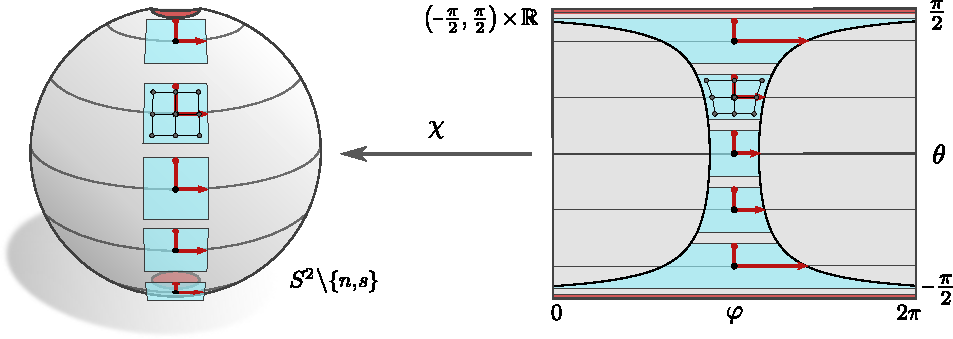
\includegraphics[width=.90\textwidth]{figures/G_structure_spherical_equirectangular_1.pdf}
    \caption{\small
        Visualization of the $\SO2$-invariant $\{e\}$-structure that is considered by most models discussed in Section~\ref{sec:spherical_CNNs_azimuthal_equivariant}.
        All of the frames 
        $\big[ \frac{\partial}{\partial\theta} ,\; \frac{1}{\cos(\theta)} \frac{\partial}{\partial\varphi} \big]$
        are aligned towards the north pole and are orthonormal w.r.t. the embedding metric of the sphere in $\R^3$.
        The spherical coordinate map
        $\chi: (-\frac{\pi}{2}, \frac{\pi}{2}) \times \R \to S^2 \backslash \{n,s\}$ from Eq.~\eqref{eq:spherical_coords}
        allows to pull spherical feature fields back to feature fields on spherical angles $(-\frac{\pi}{2}, \frac{\pi}{2}) \times \R$, which is denoted as equirectangular projection.
        Since~$\chi$ is non-isometric, the spherical $\{e\}$-structure is in coordinates deformed by a latitude dependent factor of $1/\cos(\theta)$, which diverges towards the poles.
        The spherical convolution on this $\{e\}$-structure is in~\cite{coors2018spherenet,eder2019convolutions,martin2020panoramic} implemented by projecting and interpolating a kernel sampling grid on the tangent spaces to a feature field sampling grid on the sphere.
        If the feature fields are instead sampled on the equirectangular projection, the kernel sampling grid is in a second step mapped further from the sphere to a deformed sampling grid on $(-\frac{\pi}{2}, \frac{\pi}{2}) \times \R$ \cite{zhao2018distortion,tateno2018distortion}.
        Note that regular sampling grids on the equirectangular projection oversample the signal (relative to the spherical metric) towards the poles.
    }
    \label{fig:spherical_equirectangular_1}
\end{figure}


\citet{zhao2018distortion} and \citet{tateno2018distortion} discretize their spherical feature fields $f: S^2 \backslash \{n,s\} \to \R^c$ instead in form of a regular pixel grid on an equirectangular projection of the sphere.
Mathematically, the equirectangular projection, visualized in Fig.~\ref{fig:spherical_equirectangular_1}, is formalized as the pullback
$\chi^*f = f \circ \chi: \big(\minus\frac{\pi}{2}, \frac{\pi}{2}\big) \times \R \to \R^c$,
of the image by the spherical coordinate map $\chi$ from Eq.~\eqref{eq:spherical_coords}:
\begin{equation}\label{cd:equirectangular_proj}
\begin{tikzcd}[column sep=50pt, row sep=25pt, font=\normalsize]
    {\big(\minus\frac{\pi}{2}, \frac{\pi}{2}\big)} \times \R
        \arrow[r, "\chi"]
        \arrow[rr, pos=.5, rounded corners, to path={ 
                -- ([yshift=-2.5ex]\tikztostart.south) 
                --node[below]{\small$
                    \chi^*f
                    $} ([yshift=-2.5ex]\tikztotarget.south) 
                -- (\tikztotarget.south)
                }]
    & S^2 \backslash \{n,s\}
        \arrow[r, "f"]
    & \R^c \mkern-12mu\phantom{\big)}
\end{tikzcd}
\end{equation}
As in the previous approaches, the authors project a kernel sampling grid via the gnomonic projection from the tangent spaces to the sphere.
In an additional step, they map it via $\chi$ to the equirectangular projection where they compute interpolation coefficients between the projected kernel sampling grid and the feature field sampling gird.
Since the deformation incurred by the equirectangular projection is independent from the longitude~$\phi \in \R$, it is sufficient to compute it only once for each latitude~$\theta \in {\textstyle \big(\minus\frac{\pi}{2}, \frac{\pi}{2}\big)}$.
The following diagram, which commutes by the definitions of $K^{\textup{sphere}}_p$ and $K^{\textup{equirect}}_p$, gives an overview of the gnomonic projection of a kernel $K: \R^2 \to \R^{\cout\times\cin}$ to the sphere \cite{coors2018spherenet,eder2019convolutions,martin2020panoramic} and to its equirectangular projection \cite{zhao2018distortion,tateno2018distortion} (note that $\mathscr{G}_p$ is invertible on $H_p^2$):
\begin{equation}
\begin{tikzcd}[column sep=50pt, row sep=36pt, font=\normalsize]
    & &[20pt]
    \R^{\cout\times\cin}
    \\
    \R^2
        \arrow[urr, pos=.75, rounded corners, to path={ 
                -- ([yshift=0pt]\tikztostart.north) 
                |-node[above]{\small$
                        K
                    $} ([xshift=0ex]\tikztotarget.west) 
                }]
    & \TpM
        \arrow[l, "\psiTMp^A"]
        \arrow[r, "\mathscr{G}_p = \exp_p\mkern-2mu\circ\mkern2mu\omega"']
    & H_p^2
        \arrow[u, "K_p^\textup{sphere}\,"']
    &[10pt] \underbrace{\chi^{-1}(H_p^2)}_{\subset\ (\protect\minus\frac{\pi}{2}, \frac{\pi}{2}) \times \R}
        \arrow[l, "\chi"]
        \arrow[ul, pos=.72, rounded corners, to path={ 
                -- ([yshift=0pt]\tikztostart.north) 
                |-node[above]{\small$
                    K^{\textup{equirect}}_p
                    $} ([xshift=0ex]\tikztotarget.east) 
                }]
\end{tikzcd}
\end{equation}
A major disadvantage of discretizing spherical feature fields via a regular pixel grid on the equirectangular projection is that this approach oversamples the signal towards the poles.


Further variants of spherical convolutions on the equirectangular projection were proposed by \citet{su2017spherical,su2019kernel}.
Instead of precomputing the deformed kernel sampling pattern, \citet{su2017spherical} untie the weight sharing such that each latitude applies its own, independent kernel in a 1-dimensional Euclidean convolution.
The network is then on each latitude being pretrained to recover the result that would be obtained when convolving with a kernel that is shared over the tangent spaces as discussed above.
If convolutional weight sharing is a suitable inductive bias, this method should optimally converge to the geometry based methods by \citet{zhao2018distortion,tateno2018distortion}.
\citet{su2019kernel} develop this approach further and employ a meta-network that predicts a deformed kernel based on a shared input template kernel and the target latitude.
Both of these approaches share weights over the circular orbits (lines of constant latitude) of the considered isometry group~$\SO2$ of~$S^2 \backslash \{n,s\}$; cf. Fig.~\ref{fig:isom_invariant_kernel_field_multiple_orbits}.
They are therefore identified as kernel field transforms with $\SO2$-invariant kernel fields, which are by Theorem~\ref{thm:isometry_equivariant_kernel_field_trafos} $\SO2$-equivariant.


\begin{figure}
    \centering
    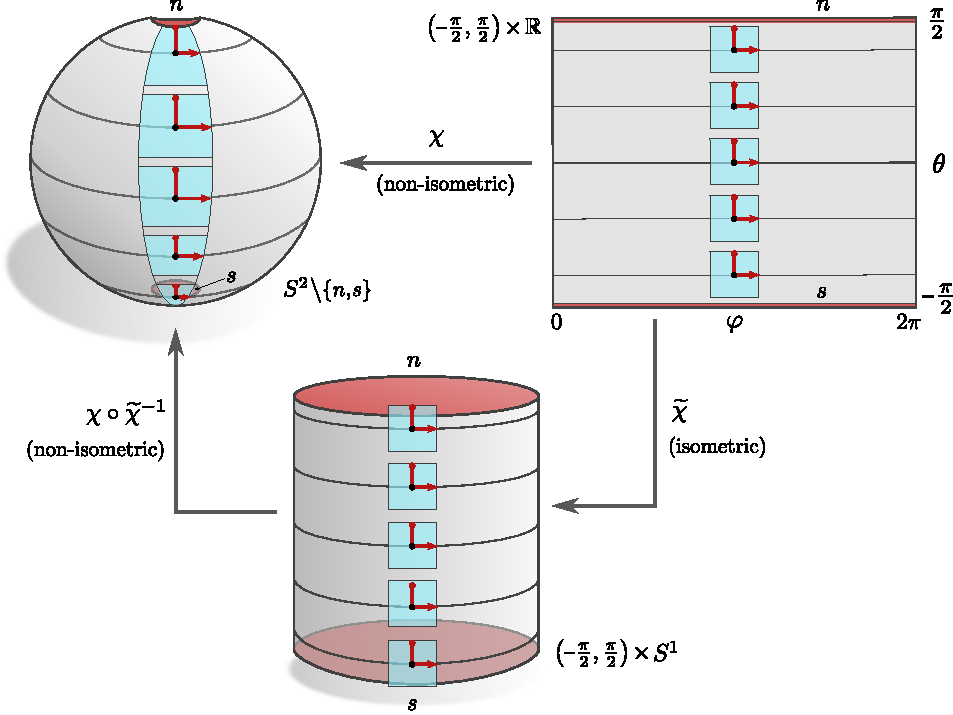
\includegraphics[width=.90\textwidth]{figures/G_structure_spherical_equirectangular_2.pdf}
    \caption{\small
        The spherical coordinate map
        $\chi: \big(\protect\minus\frac{\pi}{2}, \frac{\pi}{2}\big) \times \R \to S^2 \backslash \{n,s\}$, Eq.~\eqref{eq:spherical_coords}, sends angles $(\theta,\phi)$ to points on the sphere.
        It is non-isometric, which means that the pushforward of orthonormal frames
        $\big[ \frac{\partial}{\partial\theta}, \frac{\partial}{\partial\varphi} \big]$
        w.r.t. the \emph{Euclidean metric} on $\big(\protect\minus\frac{\pi}{2}, \frac{\pi}{2}\big) \times \R$ does not yield frames that are orthonormal w.r.t. the \emph{spherical metric}.
        A conventional Euclidean convolution in coordinates $\big(\protect\minus\frac{\pi}{2}, \frac{\pi}{2}\big) \times \R$ does therefore not correspond to a spherical convolution -- its kernels would be contracted by a factor of $\cos(\theta)$ in longitudinal direction.
        Since distances are measured in terms of angles, this operation corresponds rather to a convolution on a cylinder, which is via the isometric map
        $\widetilde{\chi}: \big( {\textstyle \protect\minus\frac{\pi}{2}, \frac{\pi}{2}} \big) \times \R
        \to \big( {\textstyle \protect\minus\frac{\pi}{2}, \frac{\pi}{2}} \big) \times S^1$,
        Eq.~\eqref{eq:cylindrical_coords}, embedded in $\R^3$.
        A spherical convolution requires the $\{e\}$-structure that is shown in Fig.~\ref{fig:spherical_equirectangular_1}.
    }
    \label{fig:spherical_equirectangular_2}
\end{figure}


Given a spherical feature field in equirectangular projection, it might
furthermore
be tempting to process it directly with a conventional Euclidean CNN, skipping the kernel projection from the tangent spaces, as done for instance in~\cite{lai2017semantic,hu2017spherical}.
As discussed in Section~\ref{sec:instantiations_euclidean}, such Euclidean convolutions correspond to $\GM$-convolutions on the canonical $\{e\}$-structure of $\big(\minus\frac{\pi}{2}, \frac{\pi}{2}\big) \times \R \subset \R^2$, visualized in Figs.~\ref{fig:G_structure_R2_1} and~\ref{fig:spherical_equirectangular_2} (top right).
This $\{e\}$-structure consists of frames 
$\big[ \frac{\partial}{\partial\theta} ,\, \frac{\partial}{\partial\varphi} \big]$,
which are orthonormal w.r.t. the \emph{Euclidean metric} of $\big(\minus\frac{\pi}{2}, \frac{\pi}{2}\big) \times \R$.
These frames are, however, not orthonormal w.r.t. the \emph{spherical metric}, Eq.~\eqref{eq:spherical_embedding_metric_explicit}, which is in Fig.~\ref{fig:spherical_equirectangular_2} (top left) reflected in the frame contraction by a factor of $\cos(\theta)$ in longitudinal direction.
A $\GM$-convolution on this $\{e\}$-structure corresponds therefore geometrically \emph{not} to a spherical convolution.
It rather corresponds to a $\GM$-convolution on a cylinder, which is via the \emph{isometric} coordinate map
\begin{align}\label{eq:cylindrical_coords}
    \widetilde{\chi}:\, \big( {\textstyle \minus\frac{\pi}{2}, \frac{\pi}{2}} \big) \!\times \R
    \,\to\, \big( {\textstyle \minus\frac{\pi}{2}, \frac{\pi}{2}} \big) \!\times S^1,
    \quad (\theta,\phi) \mapsto
    \begin{pmatrix}
        \cos{\phi} \\
        \sin{\phi} \\
        \theta
    \end{pmatrix}
\end{align}
embedded in $\R^3$.
In contrast, the $\{e\}$-structure that is shown in Figs.~\ref{fig:G_structure_S2_2} and~\ref{fig:spherical_equirectangular_1} consists of frames
$\big[ \frac{\partial}{\partial\theta} ,\; \frac{1}{\cos(\theta)} \frac{\partial}{\partial\varphi} \big]$,
which are orthonormal w.r.t. the spherical metric.
Note that these frames and the spherical metric are stretched by a factor of $1/\cos(\theta)$ relative to their canonical Euclidean counterparts on $\big( {\textstyle \minus\frac{\pi}{2}, \frac{\pi}{2}} \big) \times \R$.


\citet{jiang2019spherical} propose an alternative approach for spherical convolutions on the $\{e\}$-structure shown in Figs.~\ref{fig:G_structure_S2_2} and~\ref{fig:spherical_equirectangular_1}.
Instead of defining kernels on the tangent spaces, they process the signal via second order partial differential operators of the form $w_{\id} + w_{e^A_1} \partial_1 + w_{e^A_2} \partial_2 + w_\textup{Laplace} (\partial_1^2 + \partial_2^2)$, where $\partial_i$ denotes the partial derivative in the direction of the $i$-th frame axis and the weights $w_{(\cdot)} \in \R^{\cout\times\cin}$ are optimized during training.
That the weights are position independent corresponds to our spatial weight sharing.
Together with the $\SO2$-invariance of the $\{e\}$-structure, along which the differential operators are aligned, this guarantees the $\SO2$-equivariance of the operation.
In the continuous theory, this model corresponds to a $\GM$-convolution in the limit of infinitesimally small kernels.
In practice, \citet{jiang2019spherical} sample the feature field on an icosphere mesh and represent the differential operators in terms of spatially extended stencils on the mesh vertices.
This makes the method equivalent to a $\GM$-convolution with spatially extended kernels.


The model of \citet{lee2019spherephd} operates again on an icosphere, however, with a drastically changed (non-smooth) $\{e\}$-structure:
instead of aligning the reference frames such that they all point towards the north pole, the frames point alternatingly towards the north or south.
This design is motivated by the pixelation of the icosphere, whose triangular faces are facing either north or southwards.
Adjacent pixels can therefore be processed by kernels that are rotated by $180^\circ$ relative to each other.
The authors argue that the training process should make up for this rotation by learning accordingly steerable kernels.
Despite the drastic kernel rotations, the $\{e\}$-structure is invariant under those azimuthal rotations that map northwards pointing frames on themselves, resulting in an approximate $\SO2$-equivariance of the convolution.


The models discussed in this section are easily extended to other solids of revolution ($\SO2$-invariant manifolds) like the cylinder from Fig.~\ref{fig:spherical_equirectangular_2} or the egg from Fig.~\ref{fig:isom_egg_main}.
They are furthermore adapted to be $\O2$-equivariant when considering a lift of the $\{e\}$-structures to $\Flip$-structures, which corresponds to using $\Flip$-steerable kernels as shown in Fig.~\ref{fig:isom_invariant_kernel_field_quotient}.
